4. \begin{figure}[ht!]
\center{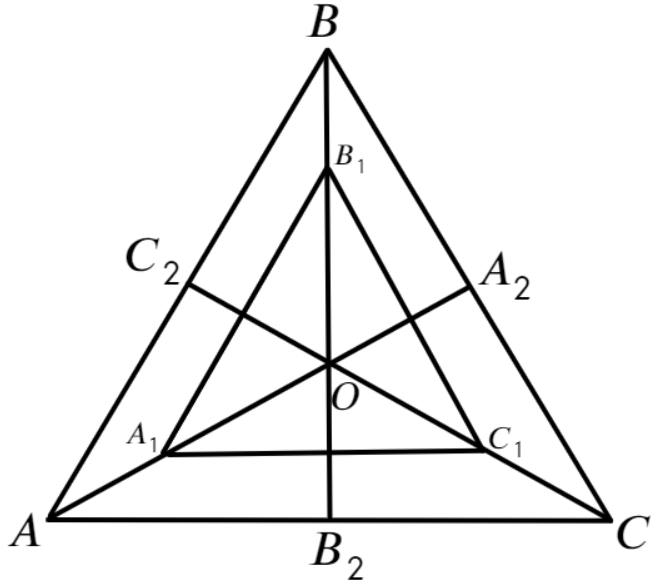
\includegraphics[scale=0.35]{g8-3.png}}
\end{figure}\\
Медианы делятся точкой пересечения в отношении $2:1,$ поэтому $AO=\cfrac{2}{3}AA_2.$ По условию $AA_1:A_1A_2=1:4,$ значит $AA_1=\cfrac{1}{5}AA_2.$ Тогда $A_1O=AO-AA_1=\cfrac{2}{3}AA_2-\cfrac{1}{5}AA_2=\cfrac{7}{15}AA_2.$ Таким образом,  $A_1O:AO=\cfrac{7}{15}AA_2:\cfrac{2}{3}AA_2=\cfrac{7}{10}$ и аналогично $B_1O:BO=C_1O:CO=\cfrac{7}{10}.$ Тогда треугольники $A_1B_1O$ с $ABO$ (а также $B_1C_1O$ с $BCO$ и $A_1C_1O$ с $ACO$) подобны по второму признаку (общий угол и одинаково относящиеся заключающие его стороны), коэффициент подобия равен $\cfrac{7}{10}.$ Тогда $S_{\Delta A_1B_1O}=\cfrac{49}{100}S_{\Delta ABO},\
S_{\Delta A_1C_1O}=\cfrac{49}{100}S_{\Delta ACO},\ S_{\Delta B_1C_1O}=\cfrac{49}{100}S_{\Delta BCO}\Rightarrow S_{\Delta A_1B_1C_1}=
S_{\Delta A_1B_1O}+S_{\Delta A_1C_1O}+S_{\Delta B_1C_1O}=\cfrac{49}{100}S_{\Delta ABO}+\cfrac{49}{100}S_{\Delta ACO}+\cfrac{49}{100}S_{\Delta BCO}=
\cfrac{49}{100}(S_{\Delta ABO}+S_{\Delta ACO}+S_{\Delta BCO})=\cfrac{49}{100}S_{\Delta ABC}.$\\
